\subsection{Determinação do calor latente de condensação da água}

O terceiro e último experimento consiste em medir o calor latente de condensação da água, $L_c$, a partir de um tubo acoplado ao calorímetro que conduz vapor de água até o seu interior. O calor latente representa a quantidade de calor necessária para que um corpo mude de fase, mantendo sua temperatura fixa e sendo proporcional à sua massa $m$. A expressão que traduz esse conceito pode ser visualizado a seguir:

\[ Q = m \cdot L\]

Sendo a constante de proporcionalidade L, denominada calor latente, uma característica da substância e do tipo de transição de fase. Com a convenção $Q>0$ quando um sistema recebe calor, e $Q<0$ quando cede, o calor latente poderá ser positivo ou negativo, dependendo da mudança de fase ocorrer com ganho ou perda de calor pelo sistema. Explicado isso, a montagem experimental descrita pode ser visualizada na imagem a seguir:

\begin{figure}[H]
  \centering
  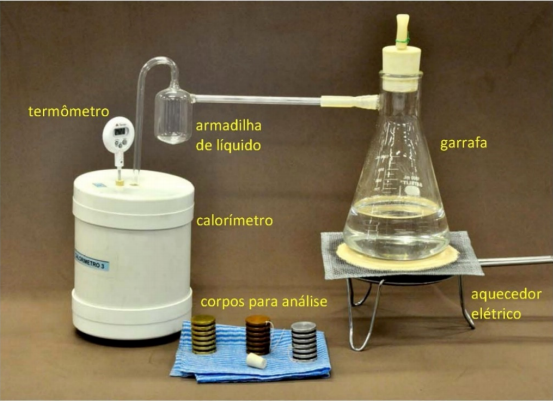
\includegraphics[scale=0.75]{images/Montagem experimental.png}
  \caption{Montagem experimental para medida do calor de vaporização da água.}
\end{figure}

Nesta imagem, pode-se observar que o calorímetro é conectado diretamente a um balão que contém água em ebulição. O elemento denominado “armadilha de líquido” é responsável por coletar o vapor que se condensou ao longo da trajetória, permitindo que apenas o vapor d’água chegue até o interior do calorímetro. Assim como nos demais experimentos, um termômetro é instalado no calorímetro para permitir que a temperatura de equilíbrio seja registrado.

Para determinar o calor latente de condensação $L_c$ da água específico, considera-se uma quantidade fixa de água de massa $m_1$ a uma temperatura $t_1$ que está em equilíbrio no interior do calorímetro com capacidade térmica $C$. Com o aquecimento da água dentro do balão, uma massa de vapor $m_2$ com temperatura $t_c$ ingressará no calorímetro até que ocorra a condensação completa.

Na situação final, o sistema completo (água, vapor condensado e calorímetro) estabiliza numa temperatura de equilíbrio em comum $t_f$. Para essa situação, as trocas de calor no processo completo satisfazem a seguinte equação:

\[ m_1 \cdot c_a \cdot (t_f - t_1) + m_2 \cdot L_c + m_2 \cdot c_a \cdot (t_f - t_c) + C \cdot (t_f - t_1) = 0\]

Em que o segundo e o terceiro termo dessa expressão estão relacionados, respectivamente, com o processo de condensação da massa $m_2$ de vapor de água e com variação de temperatura dessa mesma massa, já condensada, de $t_c$ para $t_f$. Dessa forma, pode-se chegar na seguinte expressão final para determinação do calor de condensação da água:

\[ L_c = \frac{(m_1 \cdot c_a + C) \cdot (t_1 - t_f)}{m_2} + c_a \cdot (t_c - t_f)\]

Nesse sentido, para a coleta de dados, inicialmente se aquece a água no interior do balão até atingir a temperatura de ebulição tc, sem que o tubo de vidro seja acoplado no calorímetro.

Após isso, uma massa de água $m_1$ é adicionado no interior do calorímetro para que a temperatura de equilíbrio $t_1$ seja medido pelo termômetro.

\begin{figure}[H]
  \centering
  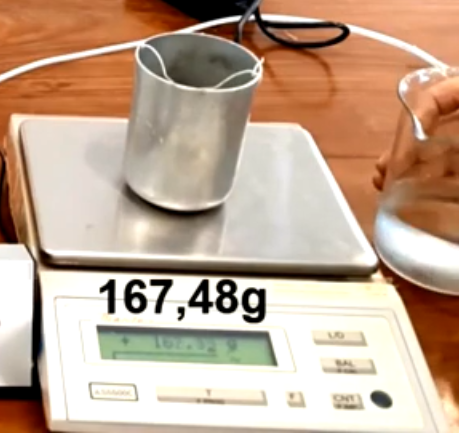
\includegraphics[scale=0.6]{images/Massa m1.png}
  \caption{Massa $m_1$ de água introduzida no interior do calorímetro.}
\end{figure}

\begin{figure}[H]
  \centering
  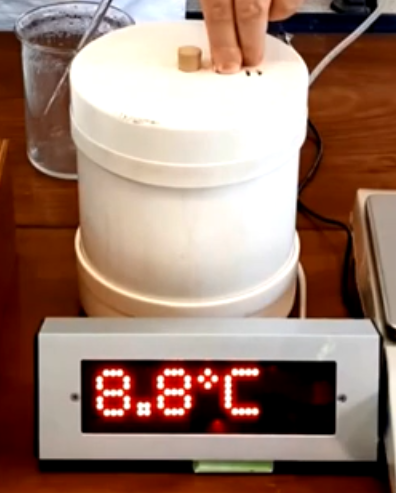
\includegraphics[scale=0.6]{images/Temperatura t1.png}
  \caption{Temperatura $t_1$ do equilíbrio no calorímetro após a adição de água fria.}
\end{figure}

Em seguida, o tubo de vidro é introduzido no interior do calorímetro, que novamente tem sua temperatura medida até cerca de 70ºC, quando equivale à entrada aproximada de 20g de vapor no interior. Então, o tubo de vidro é retirado do calorímetro, o sistema é tampado e a temperatura final $t_f$ de equilíbrio é medido.

\begin{figure}[H]
  \centering
  \includegraphics[scale=0.6]{images/Temperatura 70ºC.png}
  \caption{Registro da temperatura $t_f$ de equilíbrio após a adição de vapor d’água no interior do calorímetro.}
\end{figure}

Por fim, determina-se a massa $m_2$ de água condensada conhecendo a massa do copo do calorímetro e a massa inicial $m_1$ de água colocada. O calor latente de condensação da água $L_c$ é, então, calculado a partir da equação descrita anteriormente.

\begin{figure}[H]
  \centering
  \includegraphics[scale=0.6]{images/Massa Copo Calorímetro.png}
  \caption{Massa do copo do calorímetro.}
\end{figure}

\begin{figure}[H]
  \centering
  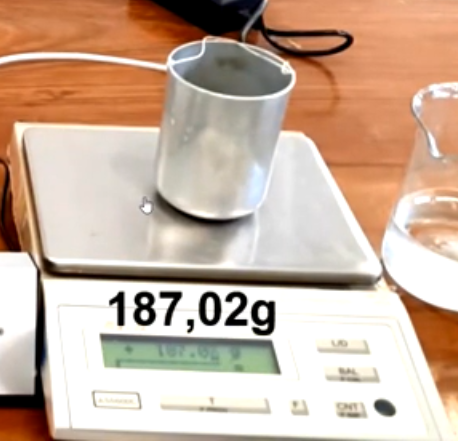
\includegraphics[scale=0.6]{images/Massa total do sistema.png}
  \caption{Massa total do sistema $m_f$ (água, vapor condensado e copo do calorímetro)}
\end{figure}
